\chapter{Effects of cell division}
\label{ch:div}

When the cell divides, all the components (organelles, proteins, genetic material, etc.) must be distributed among the daughter cells. The partition of these components is not exactly balanced. In fact, the assymetries on partition are a considerable source of noise even for components present at high numbers. In this chapter we explore some general mechanisms of partition of molecules during cell division and how they affect noise statistics.

This chapter follows the work done by D. Huh and J. Paulsson in \cite{huh11b}.

\section{Characterizing the noise arising from cell division}

Let $x = l+r$ be the number of copies of some component (e.g. a certain protein) for a dividing cell, with $l$ and $r$ being the number of copies each daughter cell recieves. Also, let $v$ be the number of molecules of some component that affects the partition such as vacuoles or spindles. On average, we expect the molecules to distribute symmetrically. Therefore
\begin{equation}
  \label{eq:div-even}
  \langle l\rangle = \langle r\rangle = \frac{\langle x\rangle}{2}.
\end{equation}

We will find the noise for $l$\footnote{It does not matter if we choose $r$ or $l$ since there is not preference for one of the daughter cells.}. Using the law of total variance [eq. \eqref{eq:con-total_var}], the variance of $l$ is given by
\begin{equation*}
  \sigma^2(l) = \sigma^2\left(\langle l|x,v\rangle\right) + \left\langle\sigma^2(l|x,v)\right\rangle.
\end{equation*}

From eq. \eqref{eq:div-even}, $\langle l|x,v\rangle = x/2$. Hence, dividing by $\langle l\rangle^2 = \langle x\rangle^2/4$ we get
\begin{equation}
  \label{eq:div-noises}
  \eta^2(l) = 4\frac{\sigma^2\left(\nicefrac{x}{2}\right)}{\langle x\rangle^2}+\frac{\langle\sigma^2(L|x,v)\rangle}{\langle L\rangle^2}=\eta^2(x) + Q_x^2,
\end{equation}

The term $Q_x$, defined as
\begin{equation}
  \label{eq:div-Q}
  Q_x^2 \coloneqq \frac{\langle\sigma^2(l|x,v)\rangle}{\langle l\rangle^2},
\end{equation}
is the noise arising from cell division. Eq. \eqref{eq:div-noises} states that the squared noise after cell division is the sum of the squared noise before division and the squared noise arising at the division process.

The term $Q_x$ can be interpreted in another way. From the definition of variance and eq. \eqref{eq:div-even}
\begin{equation*}
  Q_x^2 = \frac{1}{\langle l\rangle^2}\left\langle\left\langle\left(l-\langle l\rangle\right)^2|x,v\right\rangle\right\rangle = \frac{4}{\langle x\rangle^2}\left\langle\left\langle\left.\left(l-\frac{x}{2}\right)^2\right|x,v\right\rangle\right\rangle,
\end{equation*}
but $l - \frac{x}{2} = \frac{1}{2}(2l-(l-r)) = \frac{l-r}{2}$, then
\begin{equation*}
   Q_x^2 = \frac{4}{\langle x\rangle^2}\left\langle\left\langle\left.\left(\frac{l-r}{2}\right)^2\right|x,v\right\rangle\right\rangle  = \frac{1}{\langle x\rangle^2}\left\langle\left(l-r\right)^2\right\rangle.
\end{equation*}

Therefore, $Q_x^2$ is the average square deviation between the number of copies each daughter cell receives. For a perfect division $l=r$, making $Q_x=0$. Conversely, the most noisy case occurs when one daughter recieves all of the $x$ moleucles.

In the subsequent derivations, the diverse mechanisms related to cell division will be considered. To simplify the derivations, the particular assumptions used may not match the exact dynamics of the process, but they yield the same noise statistics. For instance, when molecules are grouped in vesicles before being segregated to each half, they are first segregated randomly into vesicles and then vesicles are distributed between the daughters. We will see that for the derivations it will be easier to invert the order of the process. Altough this does not correspond to the reality, the same noise is obtained.

\section{Independent segregation}

In the case of independent segregation, each molecule has an equal probability per unit time to migrate from a cell half to another. Assuming there are $l$ and $x-l$ molecules in each half, a process that is consistent with this supposition is
\begin{equation}
  \label{eq:div-arr_ind}
  \begin{split}
    l&\xrightarrow{x-l}l+1\\
    l&\xrightarrow{l}l-1
  \end{split}
\end{equation}

Using the FDT, the jacobian and diffusion $1\times1$ matrices are
\begin{equation*}
  \begin{split}
    \mathbf{A} &= \partial_l\left((x-l)-l\right) = -2,\\
    \mathbf{B} &= (x-l)+l = x.
  \end{split}
\end{equation*}

Solving for the covariance matrix, which in this case is the variance, we obtain in steady state
\begin{equation}
  \label{eq:div-var_ind}
  \sigma^2(l|x) = \frac{x}{4}.
\end{equation}

Averaging and using eq. \eqref{eq:div-Q} we get
\begin{equation}
  \label{div-Rindep}
  Q_x^2 = \frac{4}{\langle x\rangle^2}\left\langle\sigma^2(l|x)\right\rangle = \frac{4}{\langle x\rangle^2}\frac{\langle x\rangle}{4} = \frac{1}{\langle x\rangle}.
\end{equation}

In the following sections we find the noise for some common division mechanisms and compare it to the case of independent segregation. The mechanisms that increase the noise with respect to it were labeled by the authors as ``disordered segregation'', while those that can decrease as ``ordered segregation'' \cite{huh11b}.

\section{Disordered segregation}

\subsection{General case}

The space that is available to a component can vary between the daughter cells because there are large molecules that segregate randomly such as vacuoles. Fig. \ref{fig:div-random_volume} shows this situation.
\begin{figure}[H]
  \centering
  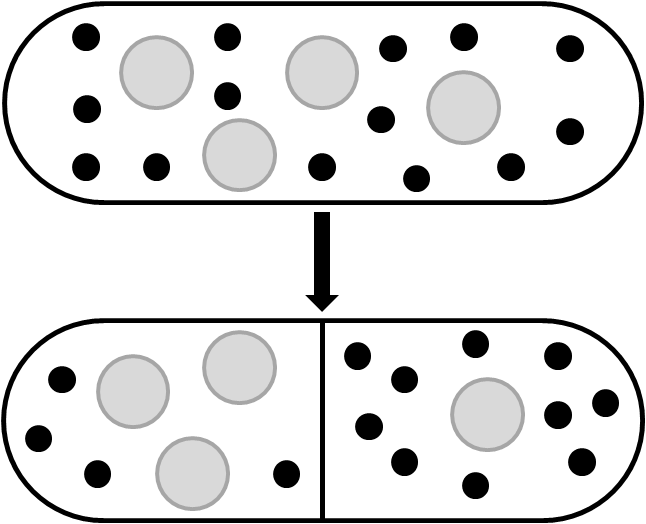
\includegraphics[width=4cm]{div-random_volume}
  \caption[Partition of molecules with random accessible volume]{\label{fig:div-random_volume}Partition of molecules with random accessible volume. The partition noise in the black molecules is increased with respect to independent segregation because there are structures (gray) that reduce the available volume in the cell.}
\end{figure}

First, we consider a general case in which the rate with which each molecules goes from a cell half to the other is proportional to the available space generated by some additional component such as vacuoles. For a fixed number $v$ of molecules of the other component, there are $n$ and $v-n$ available spaces in each daughter cell independently of $x$. Then, the process can be written as
\begin{equation}
  \label{eq:div-arr_disg}
  \begin{split}
    l&\xrightarrow{n(x-l)}l+1\\
    l&\xrightarrow{(v-n)l}l-1
  \end{split}
\end{equation}

From the law of total variance,
\begin{equation}
  \label{eq:div-varlgxv}
  \sigma^2(l|x,v) = \left\langle\sigma^2(l|x,v,n)\right\rangle_{(n|v)}+\sigma^2\left(\langle l|x,v,n\rangle\right)_{(n|v)},
\end{equation}
where the subscript $(n|v)$ denotes that averages and variances are evaluated over the conditional PMF of $n$ given $x$. Notice that taking averages over $(n|v)$ and over $(n|x,v)$ is the same in this case by the assumption that $n$ is independent of $x$. Also, by symmetry we can assume that $\langle n|v\rangle = \frac{v}{2}$.

By finding the first and second moments of $(l|x,v,n)$, we can use eq. \eqref{eq:div-varlgxv} to find its variance. The ME for its PMF $P(l|x,v,n)$ is
\begin{equation*}
  \dot{P}(l|x,v,n) = n(x-(l-1))P(l-1|x,v,n) - (v-n)lP(l|x,v,n).
\end{equation*}

Recall that the moment generating function is given by
\begin{equation}
  \label{eq:div-Gdef}
  G(z) \coloneqq \sum_{l=0}^xz^lP(l|x,v,n).
\end{equation}

The master eq. in terms of $G$ is thus given by
\begin{equation*}
  \dot{G}(z) = nxzG(z) - (v-n+nz)z\frac{\partial G(z)}{\partial z}
\end{equation*}

Hence, in steady state
\begin{equation*}
  \frac{\partial G(z)}{\partial z} = \frac{nxz}{(v-z+nz)z}G(z).
\end{equation*}

Solving with the boundary condition $G(1) = 1$, which follows from the normalization of the PDF, we find
\begin{equation*}
  G(z) = \left(1+\frac{n}{v}\left(s-1\right)\right)^x = \sum_{l=0}^x {x\choose l}\left(\frac{n}{v}\right)^l\left(1-\frac{n}{v}\right)^{x-l}z^l.
\end{equation*}

Comparing with eq. \eqref{eq:div-Gdef},
\begin{equation*}
  P(l|x,v,n) = {x\choose l}\left(\frac{n}{v}\right)^l\left(1-\frac{n}{v}\right)^{x-l},
\end{equation*}
which is a binomial distribution. Its average and variance are given by\footnote{In this case it was easy to find the PMF from the moment generating function, but we could have found the moments by differentiating and using the properties of $G$ as well.}
\begin{equation*}
  \langle l|x,v,n\rangle = \frac{n}{v}x, \quad\quad \sigma^2(L|x,v,n) = \frac{n}{v}\left(1-\frac{n}{v}\right)x.
\end{equation*}

Taking the average of the conditional variance we get
\begin{equation*}
  \begin{split}
    \left\langle\sigma^2(l|x,v,n)\right\rangle_{(n|v)} &= \left\langle\left.\frac{n}{v}\left(1-\frac{n}{v}\right)x\right|x,v,n\right\rangle_{(n|v)} = \left\langle\left.\left(\frac{n}{v}-\frac{n^2}{v^2}\right)x\right|x,v,n\right\rangle_{(n|v)}\\
    &= \left(\frac{\langle n|v\rangle}{v}-\frac{\sigma^2(n|v) + \langle n|v\rangle^2}{v^2}\right)x
  \end{split}
\end{equation*}

In the last step we replaced $\langle n^2|v\rangle = \sigma^2(n|v) + \langle n|v\rangle^2$. Since $\langle n|v\rangle = v/2$
\begin{equation}
  \label{eq:div-varofavel}
  \left\langle\sigma^2(l|x,v,n)\right\rangle_{(n|v)} = \left(\frac{1}{2} - \frac{\sigma^2(n|v)}{v^2} + \frac{1}{4}\right)x = \frac{x}{4}\left(1-Q_v^2\right),
\end{equation}
where $Q_v^2 \coloneqq 4\sigma^2(n|v)/v^2$ is the partitioning error of the relative available volume. On the other hand, the variance of the conditional mean is given by
\begin{equation}
  \label{eq:div-aveofvarl}
  \sigma^2\left(\langle l|x,v,n\rangle\right)_{(n|v)} = \sigma^2\left(\frac{n}{v}x\right)_{(n|v)} = \frac{x^2}{v^2}\sigma^2(n|v) = \frac{x^2}{4}Q_v^2.
\end{equation}

Replacing eqs. \eqref{eq:div-varofavel} and \eqref{eq:div-aveofvarl} on eq. \eqref{eq:div-varlgxv} we get
\begin{equation*}
  \sigma^2(l|x,v) = \frac{x}{4}(1-Q_v^2)+\frac{x^2}{4}Q_v^2,
\end{equation*}
and averaging and multiplying by $4/\langle x\rangle^2$
\begin{equation}
  \label{eq:div-Qdis}
  Q_x^2 = \frac{4}{\langle x\rangle^2}\left\langle\sigma^2(l|x,v)\right\rangle = \frac{4}{\langle x\rangle^2}\frac{1}{4}\left\langle x(1-Q_v^2) + x^2Q_v^2 \right\rangle = \frac{1}{\langle x\rangle} - \frac{\langle Q_v^2x\rangle}{\langle x\rangle^2} + \frac{\langle Q_v^2x^2\rangle}{\langle x\rangle^2}.
\end{equation}

We will use this equation to calculate the partitioning error $Q_x^2$ at different scenarios.

\subsection{Random size and random accessible volume}

The accessible volume for the molecules in each daughter cell can also fluctuate because the position of the septum (the division that produces the two daughter cells) is random as can be seen on fig \ref{fig:div-random_size}. This can be seen as an special case of the previous section in which there is only one volume excluding unit.
\begin{figure}[H]
  \centering
  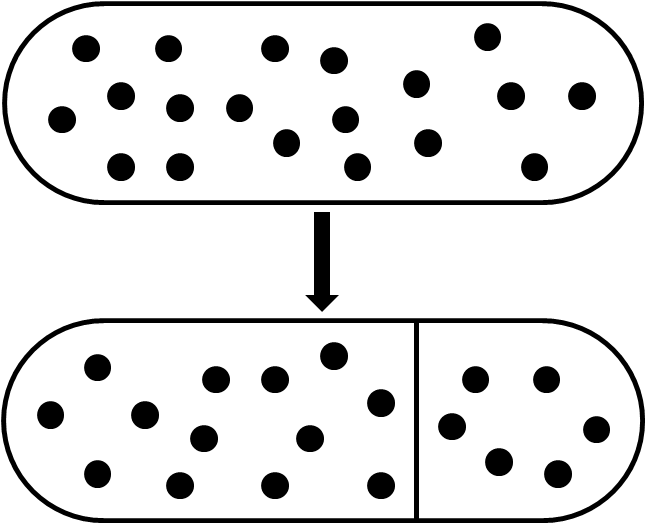
\includegraphics[width=4cm]{div-random_size}
  \caption[Partition of molecules with random size of the daughter cells]{\label{fig:div-random_size}Partition of molecules when the position of the septum is random producing daughter cells with different sizes.}
\end{figure}

Consider an available volume for the molecules that varies randomly. Let $n$ be the fraction of available volume in one of the daughter cells and assume that each molecule is equally likely to occupy any volume unit. Hence, the probability per unit time of each molecule leaving its cell half is proportional to the available volume in the other cell half. A process consistent with these suppositions is
\begin{equation*}
  \begin{split}
    l&\xrightarrow{n(x-l)}l+1\\
    l&\xrightarrow{(1-n)l}l-1
  \end{split}
\end{equation*}

This is the general case with $v=1$. Assuming the volume variance is independent of $x$, eq. \eqref{eq:div-Qdis} becomes
\begin{equation*}
  Q_x^2 = \frac{1}{\langle x\rangle} - \frac{Q_v^2}{\langle x\rangle^2}\left(\langle x\rangle  - \langle x^2\rangle\right) = \frac{1}{\langle x\rangle}\left(1-\langle Q_v^2\rangle\right) + \langle Q_v^2\rangle\frac{\langle x^2\rangle}{\langle x\rangle^2},
\end{equation*}
but $\frac{\langle x^2\rangle}{\langle x\rangle^2} = \frac{\sigma^2(x) + \langle x\rangle^2}{\langle x\rangle^2} = \eta_x^2 + 1$. Recall the definition  $Q_v^2 \coloneqq \frac{4\sigma^2(n|v)}{v^2}$. In this case $v$ is fixed at $1$. Then, $Q_{v=1}^2 = \langle Q_{v=1}^2\rangle = \sigma^2(n)/\langle n\rangle^2$, and defining $Q^2_\text{vol}\coloneqq Q_{v=1}^2$ we obtain
\begin{equation}
  \label{eq:div-Rrandom_vol}
  Q_x^2 = \frac{1-Q_\text{vol}^2}{\langle x\rangle} + Q_\text{vol}^2(\eta^2_x+1).
\end{equation}
\begin{figure}[H]
  \centering
  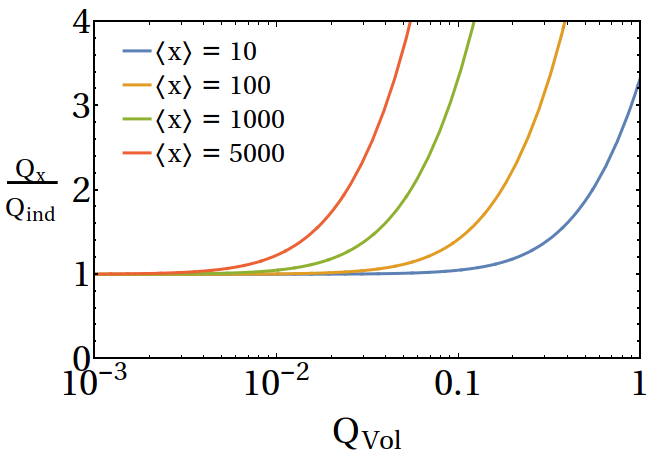
\includegraphics[width=13cm]{div-Prandom_size}
  \caption[Partition noise when the sizes of the daughter cells are random]{\label{fig:div-Prandom_size}Plot of $Q_X/Q_\text{ind}$ vs. $Q_\text{vol}$ with $Q_x$ given by eq. \eqref{eq:div-Rrandom_vol} and $Q_\text{ind}$ by eq. \eqref{div-Rindep} for two values of $\langle x\rangle$. $x$ is assumed to follow a Poisson distribution, so $\eta_x^2=1/\langle x\rangle$.}
\end{figure}

Figure \ref{fig:div-Prandom_size} shows the partition error with respect to independent segregation. For a fixed value of $Q_\text{vol}$, segregation is more disordered for larger values of $\langle x\rangle$ compared to independent segregation. Besides, in the experimentally measured range for $Q_\text{vol}$ of about $0.03 - 0.07$ \cite{huh11b}, the authors argued that variations in volume have a small impact on partition errors because they only showed the plots for $\langle x\rangle = 10$ and $\langle x\rangle = 100$. However, as we saw in chapter \ref{ch:master}, the stationary number of molecules of a protein could be in the order of $1000$ to $10000$, and with such numbers the error is considerably larger.

\subsection{Clustered segregation}

The clustering of molecules into vesicles could increase randomness in cell division. As can be seen on fig. \ref{fig:div-clustering}. There are two process that contribute to partition noise: the segregation of the molecules into the clusters, and the segregation of clusters into each daughter cell.
\begin{figure}[H]
  \centering
  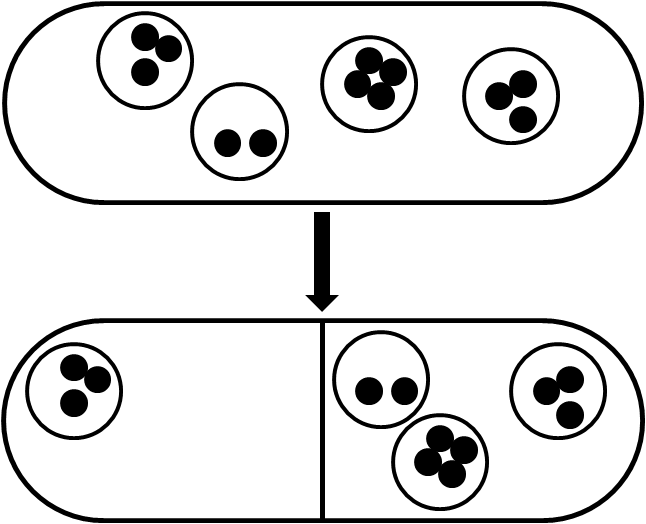
\includegraphics[width=4cm]{div-clustering}
  \caption[Partition of molecules in clusters]{\label{fig:div-clustering} Partition of molecules in clusters.}
\end{figure}

To model this mechanism, let $x$ and $v$ be the total number of molecules and vesicles in a cell before division, respectively, and let $x_i$ be the number of molecules in vesicle $i$, then $\sum_{i=0}^vx_i=x$. There are two processes that produce randomness: the migration of the molecules between vesicles and the partition of the vesicles into each daughter cells.

In the first process, a vesicle loses a molecule with a probability proportional to its number of molecules, i.e.
\begin{equation}
  \label{eq:div-vesicle_switch}
  (x_1,\dotsc,x_i,\dotsc,x_j,\dotsc x_v) \xrightarrow{x_i} (x_1,\dotsc,x_i-1,\dotsc,x_j+1,\dotsc, x_v),\quad \text{for all } j\neq i.
\end{equation}

In the second part, let $n$ be the number of vesicles in one of the daughters, then
\begin{equation}
  \label{eq:div-arr_clust}
  \begin{split}
    n &\xrightarrow{v-n} n+1,\\
    n &\xrightarrow{n} n-1.
  \end{split}
\end{equation}

If we assume both processes are independent, they can be done in any order to calculate the analytical expressions. i.e. it is the same to first distribute the molecules in each vesicle and then distribute the vesicles into each cell than to first distribute the empty vesicles between cells and then distribute the molecules. We will follow the second approach.

Let $x_1,\dotsc,x_n$ be the number of molecules in each of the vesicles of one of the daughter cells and $x_{n+1},\dotsc,x_v$ be the number of molecules in the vesicles of the other daughter cell. As usual, let $l$ be the number of molecules in one of the cells, then $l = \sum_{i=1}^nx_i$, and $r = x-l = \sum_{i=n+1}^vx_i$. Therefore, among all the possible transitions of eq. \eqref{eq:div-vesicle_switch}, the transitions from $x_i$ into $x_j$, for $i,j=1,\dotsc,n$, or $i,j=n+1,\dotsc,v$, both with $i\neq j$ does not change the number of molecules. The net effect on the number of molecules in one of the daughter cells is given by
\begin{equation*}
  \begin{split}
    l&\xrightarrow{n(x_{n+1}+\dotsb+x_{v})}l+1,\\
    l&\xrightarrow{(v-n)(x_1+\dotsb+x_n)}l-1,
  \end{split}
\end{equation*}

This is equivalent to
\begin{equation*}
  \begin{split}
    l&\xrightarrow{n(x-l)}l+1,\\
    l&\xrightarrow{(v-n)l}l-1,
  \end{split}
\end{equation*}
which is the same as eq. \eqref{eq:div-arr_disg}. Hence, from eq. \eqref{eq:div-Qdis}
\begin{equation}
  \label{eq:div-clus-Qx1}
  Q_x^2 = \frac{1}{\langle x\rangle} - \frac{\langle Q_v^2x\rangle}{\langle x\rangle^2} + \frac{\langle Q_v^2x^2\rangle}{\langle x\rangle^2}.
\end{equation}

Also, a correspondence can be established between eq. \eqref{eq:div-arr_ind} and eq. \eqref{eq:div-arr_clust} by replacing $l$ by $n$ and $x$ by $v$. Replacing on eq. \eqref{eq:div-var_ind} we get
\begin{equation*}
  \sigma^2(n|v) = \frac{v}{4}.
\end{equation*}

Recalling that $Q_v^2 \coloneqq \frac{4\sigma^2(n|v)}{v^2}$ we have in this case
\begin{equation*}
  Q_v^2 = \frac{4}{v^2}\frac{v}{4} = \frac{1}{v},
\end{equation*}
and replacing on eq. \eqref{eq:div-clus-Qx1},
\begin{equation}
  \label{eq:div-clus-Qx2}
  Q_x^2 = \frac{1}{\langle x\rangle} + \frac{1}{\langle x\rangle^2}\left(\left\langle \frac{x^2}{v}\right\rangle-\left\langle \frac{x}{v}\right\rangle \right)
\end{equation}

If $x$ and $v$ are independent we can simplify further
\begin{equation}
  \label{eq:div-Qx_vesic_almost}
  \begin{split}
    Q_x^2 &= \frac{1}{\langle x\rangle} - \frac{1}{\langle x\rangle}\left\langle\frac{1}{v}\right\rangle + \frac{\langle x^2\rangle}{\langle x\rangle^2}\left\langle\frac{1}{v}\right\rangle = \frac{1}{\langle x\rangle}\left(1-\left\langle\frac{1}{v}\right\rangle\right)+\frac{\langle x^2\rangle}{\langle x\rangle^2}\left\langle\frac{1}{v}\right\rangle\\
  &\approx \frac{1}{\langle x\rangle} + \frac{\langle x^2\rangle}{\langle x\rangle^2}\left\langle\frac{1}{v}\right\rangle = \frac{1}{\langle x\rangle} + \left(1+\eta_x^2\right)\left\langle\frac{1}{v}\right\rangle,
  \end{split}
\end{equation}
under the assumption that $\langle 1/v\rangle \ll 1$. This also allow us to do a Taylor expansion of $\langle 1/v\rangle$ about $\langle v\rangle$ obtaining
\begin{equation*}
  \begin{split}
    \left\langle\frac{1}{v}\right\rangle &\approx \left\langle \frac{1}{\langle v\rangle} - \frac{v-\langle v\rangle}{\langle v\rangle^2} + \frac{(v-\langle v\rangle)^2}{\langle v\rangle^3}\right\rangle\\
    &=\frac{1}{\langle v\rangle} + \frac{\left\langle(v-\langle v\rangle)^2\right\rangle}{\langle v\rangle^3} = \frac{1}{\langle v\rangle}\left(1+\eta_v^2\right).
  \end{split}
\end{equation*}

By replacing in eq. \eqref{eq:div-Qx_vesic_almost} we obtain an approximate expression for the partition noise
\begin{equation}
  \label{eq:div-Rclust}
  Q_x^2 \approx \frac{1}{\langle x\rangle} + \frac{(1+\eta_x^2)(1+\eta_v^2)}{\langle v\rangle}.
\end{equation}

When $x\gg 1$, $Q_x^2\approx(1+\eta_v^2)/\langle v\rangle$, meaning that the segregation of clusters is the more significant factor on partitioning error. Figure \ref{fig:div-Pclustering} shows the partition error compared to independent segregation. Different from the case of random accessible volume, segregation can be highly disordered if the mean number of clusters $\langle v\rangle$ is small and the mean number of molecules $\langle x\rangle$ is large.
\begin{figure}[H]
  \centering
  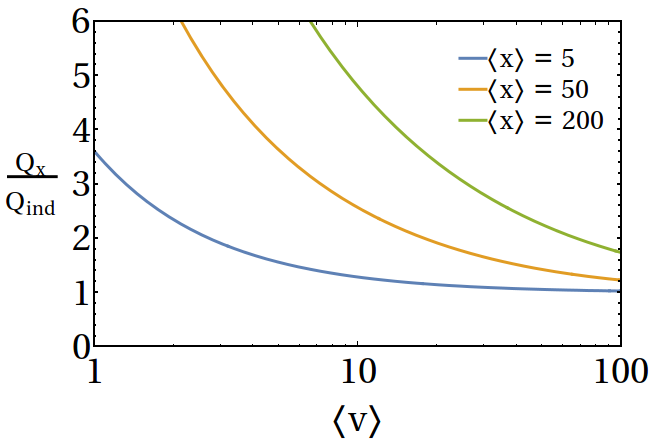
\includegraphics[width=13cm]{div-Pclustering}
  \caption[Partition noise when molecules form clusters as a function of the mean number of clusters]{\label{fig:div-Pclustering} Partition noise $Q_X$ when molecules form clusters [eq. \eqref{eq:div-Rclust}] normalized by the partition error of independent segregation $Q_\text{ind}$, as a function of $\langle v\rangle$ for three values of $\langle x\rangle$. It is assumed that $v$ and $x$ follow a Poisson distribution.}
\end{figure}

From the previous figure, we expect the degree of disorder to increase with the number of molecules. To evidence this, assume that $\langle x|v\rangle = sv$ where $s$ is a constant representing the average number of molecules per vesicle. The term in parentheses of eq. \eqref{eq:div-clus-Qx2} becomes
\begin{equation*}
  \begin{split}
    \left\langle \frac{x^2}{v}\right\rangle-\left\langle \frac{x}{v}\right\rangle &= \sum_{x,v}\left( \frac{x^2}{v}- \frac{x}{v}\right)P(x,v) = \sum_v\frac{1}{v}\left[\sum_x\left(x^2- x\right)P(x|v)\right]P(v)\\
    &=\sum_v\frac{1}{v}\left(\langle x^2|v\rangle - \langle x|v\rangle\right)P(v)=\sum_v\frac{1}{v}\left(\sigma^2(x|v) + \langle x|v\rangle^2-\langle x|v\rangle\right)P(v)\\
    &=\sum_v\frac{1}{v}\left(\frac{sv\sigma^2(x|v)}{\langle x|v\rangle} + s^2v^2-sv\right)P(v) = s\left\langle\frac{\sigma^2(x|v)}{\langle x|v\rangle}\right\rangle + s^2\langle v\rangle - s
  \end{split}
\end{equation*}

Defining $q\coloneqq\sigma^2(x|v)/\langle x|v\rangle$ and recalling that by the law of total expectation $\langle x\rangle = \left\langle\langle x|v\rangle\right\rangle = \langle sv\rangle =s\langle v\rangle$, we get
\begin{equation*}
  \left\langle \frac{x^2}{v}\right\rangle-\left\langle \frac{x}{v}\right\rangle = s\langle x\rangle+s(q-1).
\end{equation*}

Replacing in eq. \eqref{eq:div-clus-Qx2} we get
\begin{equation*}
  Q_x^2 = \frac{1}{\langle x\rangle} + \frac{1}{\langle x\rangle^2}\left(s\langle x\rangle+s(q-1)\right),
\end{equation*}
and if $(1-q)$ is very small we can approximate it as
\begin{equation}
  \label{eq:Rclust2}
  Q_x^2 \approx \frac{1}{\langle x\rangle} + \frac{s}{\langle x\rangle}.
\end{equation}

This result is exact if given $v$, $x$ follows a Poisson distribution. Figure \ref{fig:div-Pclustering2} shows the degree of segregation disorder as a function of $s$. It increases with $s$ because if $\langle x\rangle$ is large, $Q_\text{ind}$ is small. But if the same number of molecules are segregated into a small number of clusters, the partition noise of the clusters contributes greatly to the total regardless of the number of molecules.
\begin{figure}[H]
  \centering
  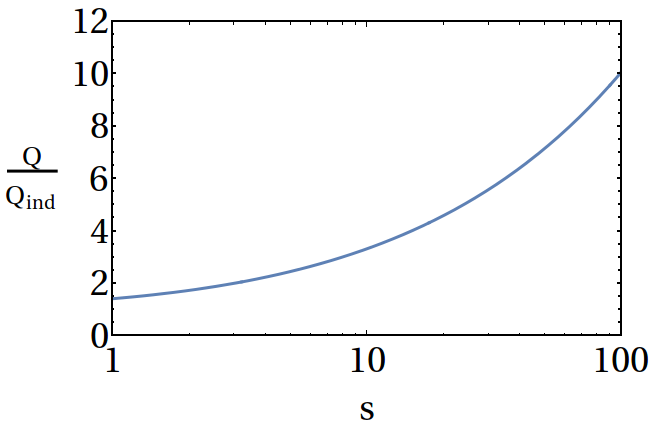
\includegraphics[width=13cm]{div-Pclustering2}
  \caption[Partition noise when molecules form clusters as a function of the number of molecules per cluster]{\label{fig:div-Pclustering2}Partition noise $Q_X$ when molecules form clusters [eq. \eqref{eq:Rclust2}] normalized by the partition error of independent segregation $Q_\text{ind}$, as a function of the the mean number of molecules per cluster $s$. It is assummed that $x|v$ follows a Poisson distribution. The curve corresponds to all values of $\langle x\rangle$.}
\end{figure}

\subsection{Upper limit of the partitioning error}

There is an upper bound for the partitioning error corresponding to the case when all the molecules migrate to one of the daughter cells. There is an equal probability for each daughter to keep all of them, thus
\begin{equation*}
  \sigma^2(l|x) = \left\langle\left(l-\frac{x}{2}\right)^2\right\rangle = \frac{1}{2}\left(0-\frac{x}{2}\right)^2+\frac{1}{2}\left(x-\frac{x}{2}\right)^2 = \frac{x^2}{4}
\end{equation*}

Therefore
\begin{equation*}
  Q_x^2 = \frac{4}{\langle x\rangle^2}\left\langle\sigma^2(l|x)\right\rangle = \frac{4}{\langle x\rangle^2}\frac{\langle x^2\rangle}{4} = \eta_x^2+1.
\end{equation*}

It depends on the heterogeneity of the mother cell.

\section{Ordered segregation}

We consider three mechanisms that reduce partitioning noise: self-volume exclusion, binding to spindles, and pair formation.

\subsection{Self-volume exclusion}

If the molecules to be segregated occupy a large volume, partition noise is reduced because parts of the cell with fewer copies have more available space (\ref{fig:div-vol_exclusion}).
\begin{figure}[H]
  \centering
  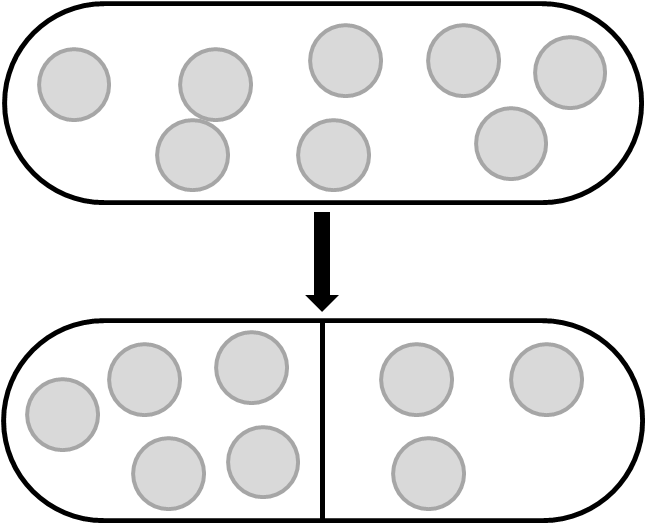
\includegraphics[width=4cm]{div-vol_exclusion}
  \caption[Partition with size exclusion]{\label{fig:div-vol_exclusion} Partition of molecules when their volumes are sufficiently large to have an effect in the available space.}
\end{figure}

Suppose that each molecule occupies a fixed fraction $k$ of the total cell volume. Also, assume that each volume unit is equally likely to be occupied by one of the copies of the molecule. The following model satisfies this supposition
\begin{equation*}
  \begin{split}
  l&\xrightarrow{(\frac{1}{2}-kl)(x-l)}l+1,\\
  l&\xrightarrow{(\frac{1}{2}-k(x-l))l}l-1.
  \end{split}
\end{equation*}

It assumes that each daughter cell has exactly $1/2$ of the total cell volume. Also, the probability for a molecule to leave its cell half its proportional to the available volume in the other cell half and the number of molecules in its cell half.

The $1\times 1$ matrices of the FDT are given by
\begin{equation*}
  \begin{split}
  \mathbf{A}&=\frac{\partial}{\partial l}\left[\left(\frac{1}{2}-kl\right)\left(x-l\right)-\left(\frac{1}{2}-k\left(x-l\right)\right)l\right]=-1,\\
  \mathbf{B}&=\left[\left(\frac{1}{2}-kl\right)\left(x-l\right)+\left(\frac{1}{2}-k\left(x-l\right)\right)l\right]_{l=\langle l|x\rangle} = \left[\frac{1}{2}x-2kxl+2kl^2\right]_{l=\langle l|x\rangle},
  \end{split}
\end{equation*}
and by symmetry $\langle l|x\rangle = x/2$, then
\begin{equation*}
  \mathbf{B} = \frac{1}{2}x(1-kx).
\end{equation*}

Replacing in the stationary FDT and solving for the variance, we obtain
\begin{equation*}
  \sigma^2(l|x) = \frac{1}{4}x(1-kx).
\end{equation*}

Hence,
\begin{equation}
  \label{eq:div-Rvol}
  Q_x^2 = \frac{4}{\langle x\rangle^2}\left\langle \sigma^2(l|x)\right\rangle = \frac{4}{\langle x\rangle^2}\frac{1}{4}\left(\langle x\rangle-k\langle x^2\rangle\right) = \frac{1}{\langle x\rangle} - k\frac{\langle x^2\rangle}{\langle x\rangle^2} = \frac{1}{\langle x\rangle} - k(\eta_x^2+1).
\end{equation}

Figure \ref{fig:div-Pvol_exclusion} evidences that to considerably reduce partition noise with respect to independent segregation the volume fraction occupied by each molecule must be large. This is biologically unrealistic for many types of components.
\begin{figure}[H]
  \centering
  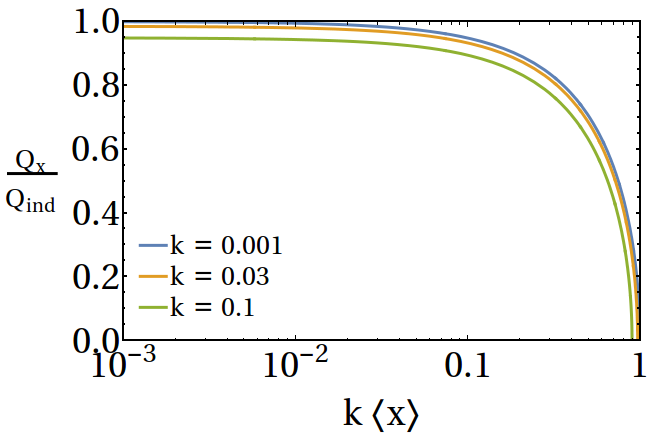
\includegraphics[width=13cm]{div-Pvol_exclusion}
  \caption[Partition noise when molecules have a non-negligible volume]{\label{fig:div-Pvol_exclusion}Partition noise $Q_x$ when molecules have a non-negligible volume [eq. \eqref{eq:div-Rvol}] normalized by the partition error of independent segregation $Q_\text{ind}$, as a function of $k\langle x\rangle$ for various values of $k$.}
\end{figure}

\subsection{Binding to spindle sites}

At the segregation process, some molecules bind to spindles that pull them to each of the daughter cells. This is characteristic for chromosome segregation during mitosis and meiosis in eukaryotes, a process that has to be very reliable. Figure \ref{fig:div-spindles} shows how this process occurs.
\begin{figure}[H]
  \centering
  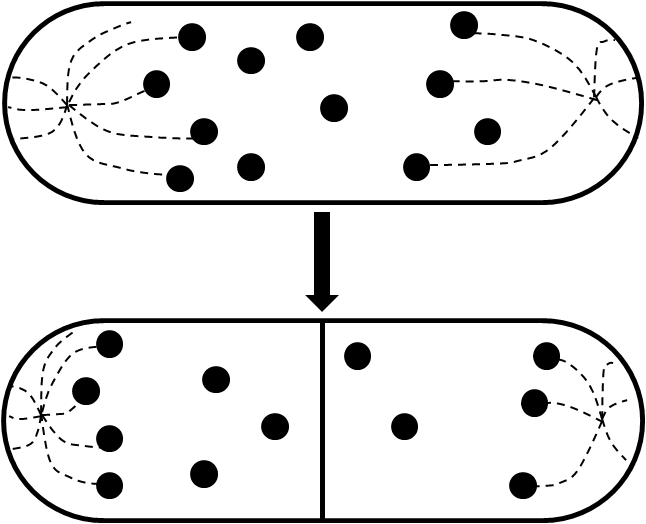
\includegraphics[width=4cm]{div-spindles}
  \caption[Partition of molecules when they bind to spindle sites]{\label{fig:div-spindles} Partition of molecules when they bind to spindle sites.}
\end{figure}

Suppose each dividing cells has a number $v$ of binding sites which are distributed randomly between both daughter cells. Let $x$ be the total number of molecules which are going to bind the sites before division. Also, assume that all possible molecules of $x$ are bound, i.e. at equilibrium if $v<x$ all binding sites are occupied, and if $v>x$ all molecules are bound.

Let $n$ be the number of binding sites on a cell half, and suppose that it increases with a rate dependent on the number of binding sites in the other cell half, then
\begin{equation*}
  \begin{split}
    n&\xrightarrow{f(v-n)}n+1,\\
    n&\xrightarrow{f(n)}n-1,
  \end{split}
\end{equation*}
where $f$ is some function. Also, the rate at which a molecule leaves a cell half is proportional to the number of molecules in its cell half and the number of free sites in the other cell half. With these assumptions the transitions for $l$ are
\begin{equation*}
  \begin{split}
    l&\xrightarrow{\lambda(n-l)(x-l)}l+1,\\
    l&\xrightarrow{\lambda(v-n-x+l)l}l-1.
  \end{split}
\end{equation*}

From the FDT, if $v\geq x$ the variance is given by
\begin{equation*}
  \sigma^2(l|x,v) =\frac{1}{4}\left(x-\frac{x^2}{v}+Q_v^2x^2\right),\quad \text{for } v\geq x,
\end{equation*}
with $Q_v^2 \coloneqq 4\sigma^2(n|v)/v^2$ as before. If $v<x$, the $v$ copies of the molecule that are bound segregate along with $n$, and for the remaining copies suppose they segregate independently. The result is
\begin{equation*}
  \sigma^2(l|x,v) = \frac{1}{4}(x-v) + \sigma^2(n|v) = \frac{1}{4}\left(x-v+v^2Q_v^2\right),\quad \text{for } v<x.
\end{equation*}

Both cases are mutually exclusive, then by definition of expected value
\begin{equation*}
  \begin{split}
    Q_x^2 &= \frac{4}{\langle x\rangle^2}\left\langle\sigma^2(l|x)\right\rangle = \frac{1}{\langle x\rangle^2}\sum_{x,v}\sigma^2(l|x)P(x,v)\\
    &=\frac{1}{\langle x\rangle^2}\left[\sum_{v\geq x}\left(x-\frac{x^2}{v}+Q_v^2x^2\right)P(x,v) + \sum_{v<x}\left(x-v+v^2Q_v^2\right)P(x,v)\right]\\,
  \end{split}
\end{equation*}
notice that there is an $x$ in both sums than can be taken out as a $\langle x\rangle$. Separating the sums by first summing $x$ and then over all $v$s we obtain
\begin{equation*}
  \begin{split}
     Q_x^2 &= \frac{1}{\langle x\rangle} - \frac{1}{\langle x\rangle^2}\sum_{v=0}^\infty\left[\sum_{x=0}^v\left(\frac{1}{v}-Q_v^2\right)x^2P(x,v)+\sum_{x=v+1}^\infty\left(v-v^2Q_v^2\right)P(x,v)\right]\\
     &=\frac{1}{\langle x\rangle} - \frac{1}{\langle x\rangle^2}\sum_{v=0}^\infty\left[\left(\frac{1}{v}-Q_v^2\right)\sum_{x=0}^vx^2P(x,v)+\left(v-v^2Q_v^2\right)\sum_{x=v+1}^\infty P(x,v)\right].
  \end{split}
\end{equation*}

Consider a simpler case in which $v$ is fixed, each daughter cell recieves exactly $v/2$ binding sites, $\langle x\rangle = v$, and $P(x)$ is symmetric. With these assumptions, the previous eq. can be reduced to
\begin{equation*}
  Q_x^2 = \frac{1}{\langle x\rangle} - \frac{1}{\langle x\rangle^2}\left[\frac{1}{v}\sum_{x=0}^vx^2P(x)+v\sum_{x=v+1}^{2v}P(x)\right].
\end{equation*}

For the sum over $v$ only survives the term corresponding to the fixed number $v$ of binding sites, and $Q_v=0$ because $n$ is now fixed. Writing $x^2 = \left(x-\langle x\rangle\right)^2 + 2x\langle x\rangle - \langle x\rangle^2$ on the first sum we get 
\begin{equation*}
  Q_x^2 = \frac{1}{\langle x\rangle}-\frac{1}{\langle x\rangle^2}\left[\frac{\sigma^2(x)}{v}\sum_{x=0}^vP(x)+\frac{2\langle x\rangle}{v}\sum_{x=0}^vxP(x)-\frac{\langle x\rangle^2}{v}\sum_{x=0}^vP(x)+v\sum_{x=v+1}^{2v}P(x)\right],
\end{equation*}
and evaluating $\langle x\rangle = v$,
\begin{equation*}
  Q_x^2 = \frac{1}{\langle x\rangle}-\frac{1}{\langle x\rangle^2}\left[\frac{\sigma^2(x)}{v}\sum_{x=0}^vP(x)+2\sum_{x=0}^vxP(x)-v\sum_{x=0}^vP(x)+v\sum_{x=v+1}^{2v}P(x)\right].
\end{equation*}

Since $P(x)$ is symmetric about $x=v$, $\sum_{x=0}^vP(x) = \sum_{x=v+1}^{2v}P(x) = 1/2$, using this
\begin{equation}
  \label{eq:div-spindles_1}
  Q_x^2 = \frac{1}{\langle x\rangle}-\frac{1}{\langle x\rangle^2}\left[\frac{\sigma^2(x)}{2v}+2\sum_{x=0}^vxP(x)\right].
\end{equation}

The absolute deviation $\left\langle\left|x-\langle x\rangle\right|\right\rangle$ can be written using the symmetry of $P(x)$ as
\begin{equation*}
  \left\langle\left|x-\langle x\rangle\right|\right\rangle = \sum_{x=0}^\infty\left|x-\langle x\rangle\right|P(x) = 2\sum_{x=0}^v\left(\langle x\rangle-x\right)P(x) = \langle x\rangle-2\sum_{x=0}^vxP(x).
\end{equation*}

Replacing this result in eq. \eqref{eq:div-spindles_1},
\begin{equation*}
  Q_x^2 = \frac{1}{\langle x\rangle}-\frac{1}{\langle x\rangle^2}\left[\frac{\sigma^2(x)}{2v}+\langle x\rangle-\left\langle\left|x-\langle x\rangle\right|\right\rangle\right] = \frac{\left\langle\left|x-\langle x\rangle\right|\right\rangle}{\langle x\rangle^2}-\frac{\eta_x^2}{2v},
\end{equation*}
and using $v=\langle x\rangle$
\begin{equation*}
  Q_x^2 = \frac{1}{\langle x\rangle}\left(\frac{\left\langle\left|x-\langle x\rangle\right|\right\rangle}{\langle x\rangle}-\frac{\eta_x^2}{2}\right).
\end{equation*}

\subsection{Pair formation mechanisms}

The molecules to be segregated can form pairs than during their partition are separated using spindles into each cell half. If the splitting process has a low error, it can reduce partition errors. Figure \ref{fig:div-pair} shows how this process occurs.
\begin{figure}[H]
  \centering
  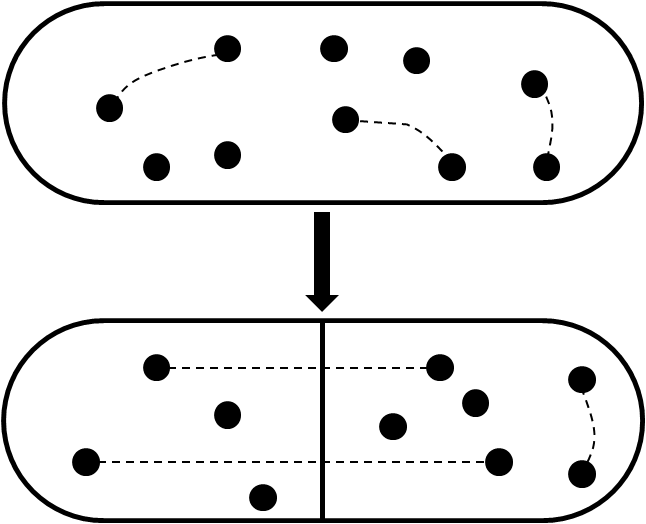
\includegraphics[width=4cm]{div-pair}
  \caption[Pair formation between molecules before segregation]{\label{fig:div-pair}Pair formation between molecules before segregation. The molecules form pairs using and then are separated into each daughter cell.}
\end{figure}

Suppose that in each cell there are $z$ pairs of molecules and $m$ independent molecules, i.e. $x=m+2z$. Also, assume that the paired molecules do not interact with the unpaired ones, then
\begin{equation}
  \label{eq:div-pu}
  \begin{split}
    \left\langle\sigma^2(l|x)\right\rangle &= \left\langle\sigma^2_\text{p}(l|2z)\right\rangle + \left\langle\sigma^2_\text{u}(l|m)\right\rangle = \sum_{x,z}\left[\sigma^2_\text{p}(l|2z) + \sigma^2_\text{u}(l|m)\right]P(2z,x)\\
    &= \sum_{x,z}\left[\sigma^2_\text{p}(l|2z) + \sigma^2_\text{u}(l|x-2z)\right]P(2z|x)P(x),
  \end{split}
\end{equation}
where the subscripts 'p' and 'u' represent the 'paired' and 'unpaired' molecules, respectively, and $P(2z,x)$ is the PMF of having $z$ pairs and a total of $x$ molecules before division. Now We will proceed to find each one of the variances. The unpaired molecules segregate independently, therefore, by comparison with eq. \eqref{eq:div-var_ind} we get
\begin{equation}
  \label{eq:div-u}
  \sigma^2_\text{u}(l|x-2z) = \frac{x-2z}{4}.
\end{equation}

For the paired molecules, assume that each pair is split to separate daughters with probability $p$ and to the same daughter with probability $1-p$. If the second case happends, there is an equal probability of ending in each daughter. Let $M$ be the number of unsorted molecules, and $L$ and $R$ the number of sorted molecules to each cell half. The sorting process of the pairs can be modeled with the following process
\begin{equation*}
  \begin{split}
    (M,l,r)&\xrightarrow{pM}(M-2,l+1,r+1),\\
    (M,l,r)&\xrightarrow{(1-p)M/2}(M-2,l+2,r),\\
    (M,l,r)&\xrightarrow{(1-p)M/2}(M-2,l,r+2),
  \end{split}
\end{equation*}
where the first line represents a succesfull split and the other two unsuccesful ones. With this relations, the matrices $\mathbf{A}$ and $\mathbf{B}$ of the time dependent FDT can be found and solved for the variances. To represent a sorting of $2z$ molecules, the initial conditions are $M(0) = 2z$, $L(0) = R(0)=0$, and all the entries of the covariance matrix are zero. The variance of the paired molecules after the sorting process is complete corresponds to the limit where the time of the process goes to infinity. After doing some algebraic steps the result is
\begin{equation}
  \label{eq:div-p}
  \sigma^2_\text{p}=(1-p)z.
\end{equation}

Replacing eqs. \eqref{eq:div-u} and \eqref{eq:div-p} in eq. \eqref{eq:div-pu} we get
\begin{equation*}
  \begin{split}
    \left\langle\sigma^2(l|x)\right\rangle &=\sum_{x}\left[\sum_z\left((1-p)z+\frac{x-2z}{4}\right)P(2z|x)\right]P(x)\\
&=\sum_x\left(\frac{1-p}{2}\langle 2z|x\rangle+\frac{x-\langle 2z|x\rangle}{4}\right)P(x)\\
    &=\frac{1}{4}\sum_x\left(2(1-p)\langle 2z|x\rangle+x-\langle 2z|x\rangle\right)P(x) = \frac{1}{4}\sum_x\left(x-(2p-1)\langle 2z|x\rangle\right)P(x)\\
    &=\frac{1}{4}\left(\langle x\rangle - (2p-1)\langle 2z\rangle\right).
  \end{split}
\end{equation*}

Hence,
\begin{equation}
  \label{eq:div-Rpair}
  Q_x^2 = \frac{1 - (2p-1)k}{\langle x\rangle},
\end{equation}
where $k\coloneqq\langle 2z\rangle/\langle x\rangle$ is the average fraction of molecules that are in pairs. If $k=0$ there is independent segregation and $Q_x = 1/\langle x\rangle$ on the previous equation. For the segregation into pairs to be ordered, $p$ must be greater than $1/2$, in the opposite case, the paired molecules have a higher chance of not being split, increasing segregation error with respect to the independent case.
\begin{figure}[H]
  \centering
  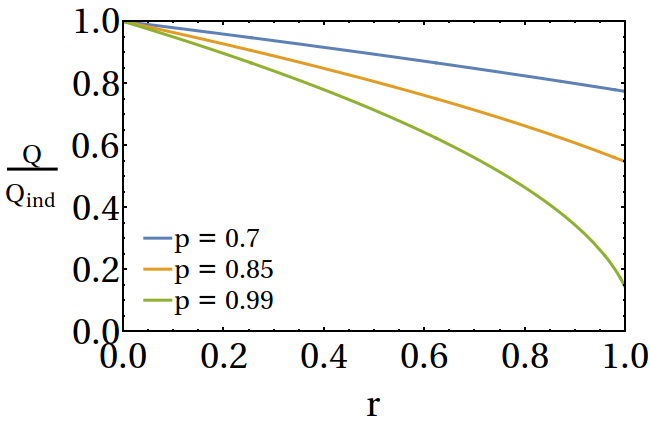
\includegraphics[width=13cm]{div-Ppair}
  \caption[Partition noise when molecules form pairs]{\label{fig:div-Ppair}Partition noise when molecules form pairs [eq. \eqref{eq:div-Rpair}] normalized by $Q_\text{ind}$ as a function of $k$.}
\end{figure}

Figure \ref{fig:div-Ppair} shows that for the partition error to be considerably reduced, the probability of a successful split $p$ should be very close to $1$ and the mean fraction of paired molecules $k$ must also be close to $1$.

\section{Final remarks}

From the analysis of the previous section, the analyzed mechanisms of ordered segregation need extreme values of the parameters to considerably reduce partition noise. Besides, we have seen that for some mechanisms, noise could be large regardless of having a high number of copies (e.g. segregation in clusters). For these reasons, partition noise is, in general, not negligible and it must be considered in the models.

Besides, to effectively reduce partition errors each source of noise must be independently controlled. For example, in the case of clustered segregation. Both the number of molecules and the number of clusters must be adjusted to avoid large errors. This is different from gene expression, in which fluctuations arising from many sources can be controlled with a single negative feedback loop. In this sense, controlling partitioning error is very difficult.

Finally, in this chapter we added more possible ways in which noise can be affected. It is then completely clear that it is impossible to infer parameters of a gene circuit based only on noise measurements and prior assumptions. For example, some of the mechanisms analyzed in this chapter produce a partition noise of the form
\begin{equation*}
  Q_x^2=\frac{A}{\langle x\rangle},
\end{equation*}
where $A$ depends on the specific mechanism. Many combinations of $A$ and $\langle x\rangle$ yield the same noise, and if the noise is measured, $A$ and $\langle x\rangle$ are not known separately. Consequently, the mechanism that produces the noise can not be inferred.
